% chapters/cap5_circuito/cap5.tex
\chapter{Diseño e Implementación del Circuito Cuántico}
\label{cap:implementacion_circuito}

En el capítulo anterior se estableció la formulación matemática para la discretización espacial de la hidrodinámica de partículas suavizadas (SPH) en un formalismo cuántico. Específicamente, se definió la construcción de una matriz hermítica, la cual actúa directamente como el hamiltoniano $H$ del sistema continuo (Continuous-Time Quantum Walk, CTQW). En el presente capítulo, se describe el proceso seguido para traducir el operador de evolución temporal a un circuito de puertas cuánticas universales.

\section{Descomposición de emparejamiento (Matching Decomposition)}
\label{sec:matching_decomposition}

La simulación de la dinámica de un sistema cuántico cerrado dictado por un hamiltoniano $H$ requiere la implementación del operador de evolución temporal $U(t) = e^{-iHt}$. En el contexto de este trabajo, $H$ corresponde a la matriz hermítica mínima a partir de adyacencia del grafo ponderado definido por las interacciones de las partículas SPH. Tradicionalmente, la simulación de estos operadores en hardware cuántico universal se realiza mediante la Descomposición de Pauli (\emph{Pauli Decomposition}). Este método estándar proyecta el hamiltoniano en una base de cadenas de operadores de Pauli $P_j \in \{I, X, Y, Z\}^{\otimes n}$, de forma que $H = \sum_{j} c_j P_j$. Sin embargo, este enfoque tiene una limitación de escalabilidad, ya que, para un grafo de $N = 2^n$ nodos, la descomposición puede generar hasta $\mathcal{O}(N^2)$ términos no locales, lo que se traduce en circuitos con una profundidad excesiva y una alta densidad de puertas $CNOT$, haciéndolos inviables en la era $NISQ$ (\emph{Noisy Intermediate-Scale Quantum}).

Para intentar abordar esta limitación y lograr un circuito viable, en este trabajo se emplea la descomposición de emparejamiento (\textit{Matching Decomposition}), propuesta en \cite{matching2026}. Este método aprovecha la topología inherente del grafo de interacciones para descomponer el hamiltoniano sin transitar por el espacio de Pauli, operando directamente sobre las aristas del grafo.

Sea $G = (V, E)$ el grafo cuyas aristas están ponderadas por el kernel SPH. Un emparejamiento o \textit{matching} $M$ se define como un subconjunto de aristas $E$ tal que ningún par de aristas en $M$ comparte un vértice común. El teorema de Vizing garantiza que las aristas de cualquier grafo con grado máximo $\Delta$ pueden ser particionadas (coloreadas) en a lo sumo $\Delta + 1$ emparejamientos disjuntos. Así, el hamiltoniano total se puede expresar como la suma de hamiltonianos parciales, cada uno correspondiente a un emparejamiento:
\begin{equation}
    H = \sum_{k=1}^{\chi} H_{M_k}
\end{equation}
donde $\chi \leq \Delta + 1$ es el índice cromático del grafo y $H_{M_k}$ contiene únicamente interacciones entre pares de vértices aislados temporalmente del resto de la red, \cite{vizing1964estimate}.

La ventaja crítica de esta formulación radica en la conmutatividad local. Dado que las aristas dentro de un mismo emparejamiento $M_k$ no comparten vértices, los operadores de evolución correspondientes a cada arista dentro de $M_k$ conmutan estrictamente entre sí. Por lo tanto, el operador de evolución temporal para el sub-hamiltoniano $H_{M_k}$ puede aplicarse de manera exacta y en paralelo:
\begin{equation}
    e^{-i H_{M_k} t} = \prod_{(u,v) \in M_k} e^{-i w_{u,v} \sigma_{x}^{(u,v)} t}
\end{equation}
donde $w_{u,v}$ representa el peso del kernel SPH entre las partículas $u$ y $v$. La transición a la evolución global del sistema se aproxima utilizando la fórmula de Trotter-Suzuki de primer orden (o superior):
\begin{equation}
    e^{-i H t} \approx \left( \prod_{k=1}^{\chi} e^{-i H_{M_k} \frac{t}{r}} \right)^r
\end{equation}
donde $r$ es el número de pasos de Trotter, \cite{suzuki1976generalized}. 

A nivel de circuito, cada interacción bidireccional entre nodos $(u,v)$ en la base computacional se implementa utilizando rotaciones controladas ($CR_x$) enmarcadas por puertas $CNOT$ para aislar el subespacio de los dos estados involucrados. Al implementar directamente la conectividad geométrica del fluido SPH, en grafos generales \textit{Matching Decomposition} puede reducir el número de operaciones de entrelazamiento. Según lo demostrado en \cite{matching2026}, este enfoque logra reducir la cantidad de puertas $CX$ hasta en un $43\%$ y acortar la profundidad del circuito en un $54\%$ frente a métodos convencionales, lo cual es interesante en este trabajo para mantener la coherencia del estado cuántico durante la simulación de la advección. Esas reducciones corresponden a los grafos estudiados por dichos autores. En el dímero de este trabajo el \textit{matching} es trivial y cada paso de Trotter se reduce a una rotación $R_x$ (figura~\ref{fig:circuito_1}); no se reporta aquí una ganancia de $CX$ propia.

\section{Primera implementación}
\label{sec:primera_implementacion}

Como primera aproximación al problema, se empleó directamente la matriz de adyacencia definida en la ecuación \ref{mat: J}, aplicando el método de \textit{Matching Decomposition} descrito en la sección \ref{sec:matching_decomposition}. Para esta simulación inicial, se adoptaron los parámetros físicos propuestos por Au-Yeung \textit{et al.} \cite{auyeung2025}: $h = 1.2$, $\Delta x = 0.5$, $c = 10^{-0.5}$ y $v = 1.0 / h^2$. La velocidad de advección $c$ fue seleccionada específicamente basándose en los experimentos de la literatura \cite{auyeung2025}, ya que promueve una mayor interacción de la cantidad advectada entre las partículas.

Al calcular los coeficientes $\alpha$ de la ecuación \ref{eq: alfa} con estos parámetros, se obtiene la siguiente matriz hermitiana $J$ para un sistema de dos partículas:

\begin{equation}
    J = 
    \begin{pmatrix}
    0 & 0.1098 \\
    0.1098 & 0
    \end{pmatrix}
    \label{mat: J_classical}
\end{equation}

Esta matriz $J$ actúa como el hamiltoniano del sistema. Para su traducción computacional, se desarrolló un algoritmo en Python utilizando la librería Qiskit, el cual implementa el pseudocódigo propuesto en \cite{matching2026}. Este programa toma la matriz y devuelve un circuito cuántico optimizado. 

Para gestionar la evolución temporal, es necesario discretizar el tiempo total de simulación mediante la fórmula de Trotter-Suzuki. Se definió un tiempo final objetivo de $t_{final} = 30$, descompuesto en $r = 100$ pasos de Trotter. Esto establece un paso de tiempo físico $\Delta t = 0.3$. De este modo, cada bloque de Trotter en el circuito representa la evolución del fluido durante un instante $\Delta t$. En la figura \ref{fig:circuito_1} se ilustra el circuito resultante para un único bloque de Trotter, el cual, gracias a la simplicidad del caso de dos partículas y la eficiencia del \textit{Matching Decomposition}, se reduce a una única puerta de rotación $R_x(0.65881)$ por cada $\Delta t$, como corresponde a un único emparejamiento en $N=2$. Para alcanzar el tiempo final $t_{final}$, este bloque debe aplicarse 100 veces.

\begin{figure}[htbp]
    \centering
    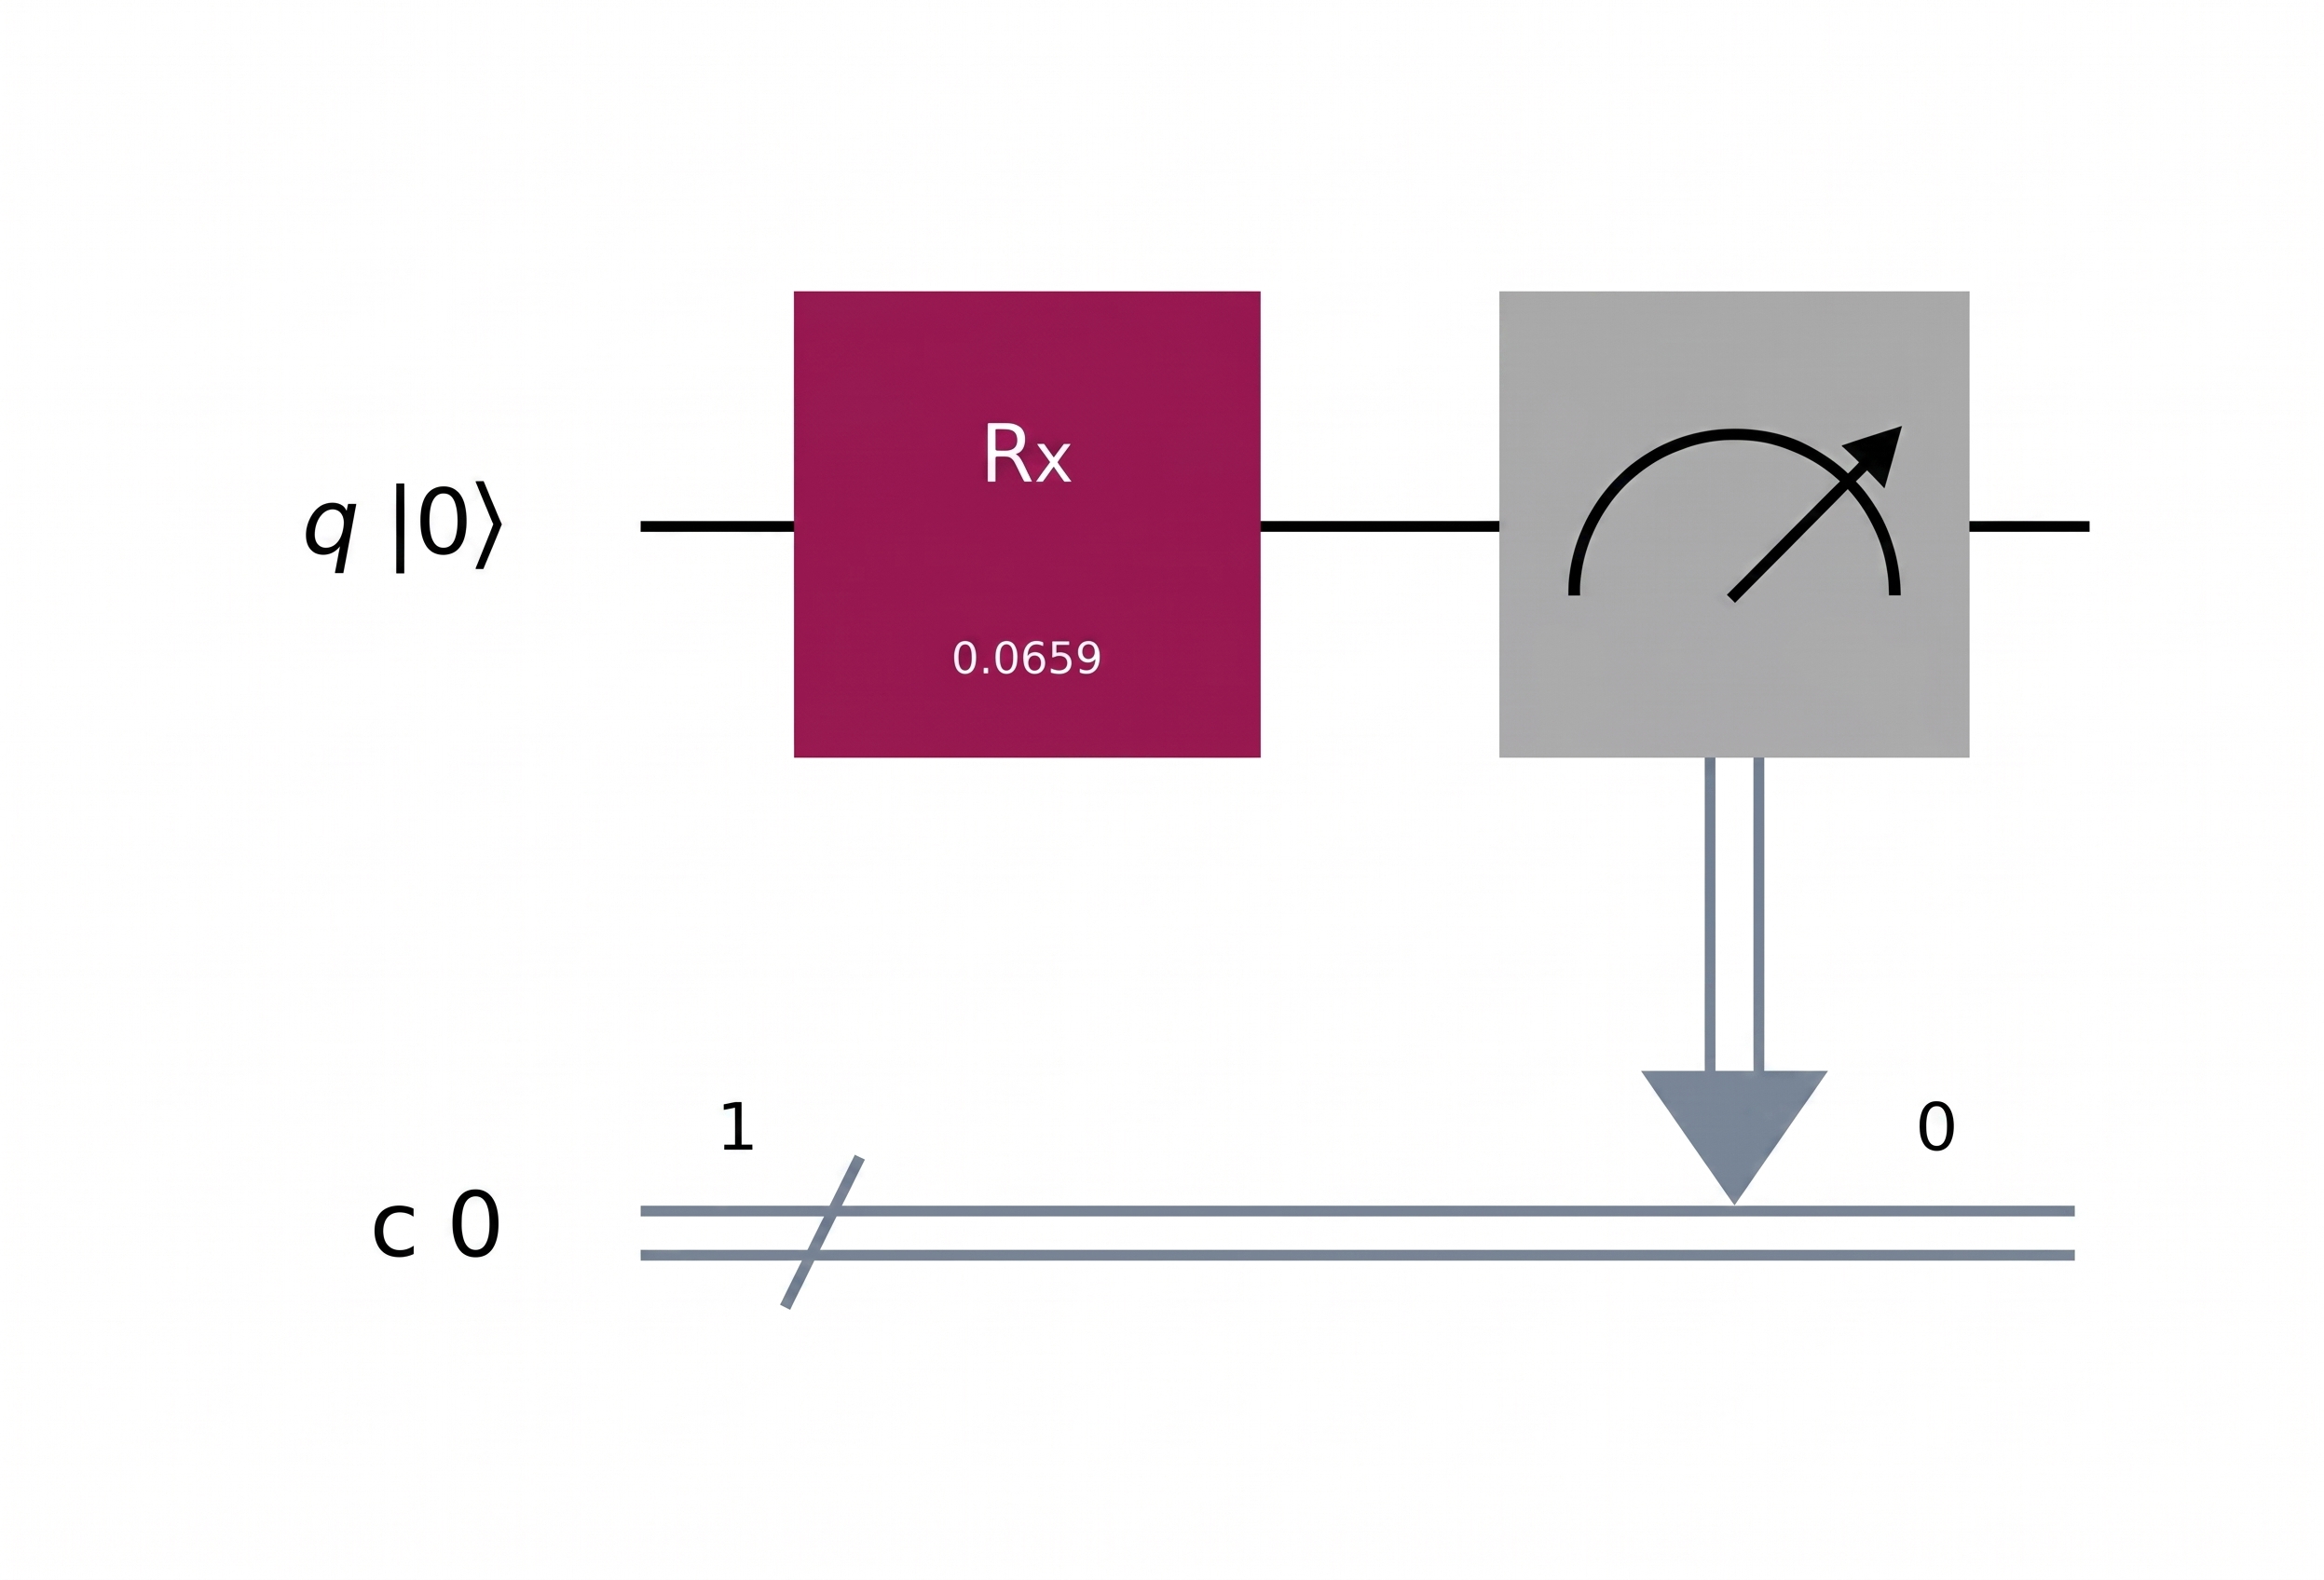
\includegraphics[width=0.6\textwidth]{chapters/cap5_circuito/img/circuito_1.png}
    \caption{Implementación de un único bloque de Trotter correspondiente a un paso de tiempo $\Delta t = 0.3$. La interacción del kernel SPH se traduce en una rotación $R_x$ sobre los qubits del sistema.}
    \label{fig:circuito_1}
\end{figure}

Para evaluar la dinámica del circuito, se realizaron simulaciones con 4000 \textit{shots} (mediciones) por cada ejecución. Con el fin de tener una resolución legible en la dinámica temporal, la gráfica se construyó muestreando únicamente 30 puntos distribuidos uniformemente a lo largo de los 100 pasos de Trotter. Los resultados se muestran en la figura \ref{fig:resultado_1}, donde se representan las poblaciones $P_j$ del qubit del sistema.

\begin{figure}[htbp]
    \centering
    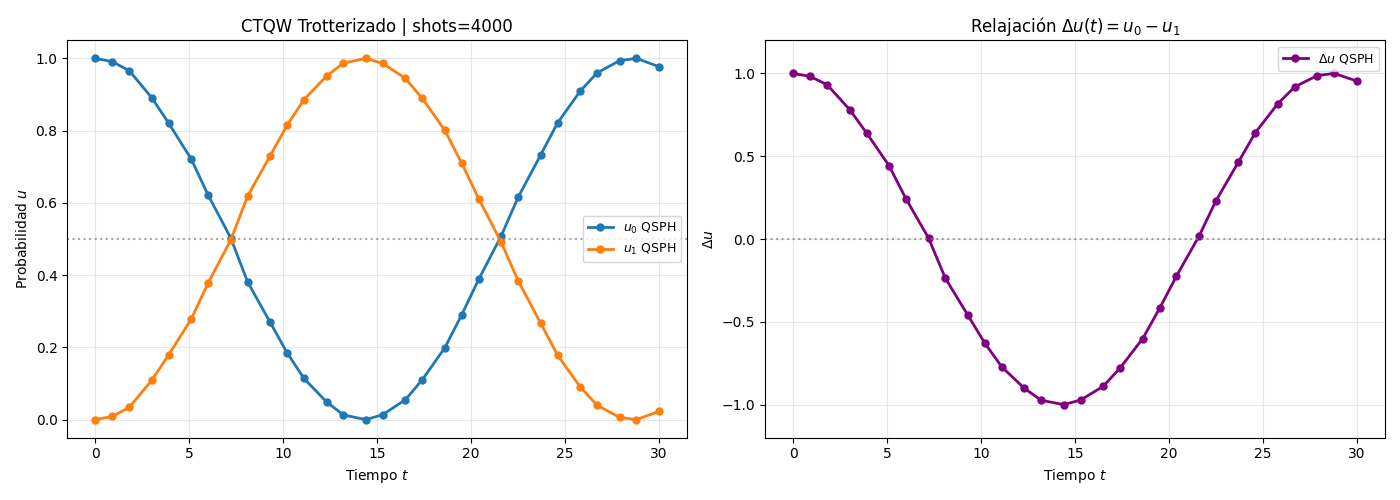
\includegraphics[width=1\textwidth]{chapters/cap5_circuito/img/resultado_1.png}
    \caption{Evolución temporal de las poblaciones $P_j$ en el circuito unitario (CTQW cerrado).}
    \label{fig:resultado_1}
\end{figure}

\subsection{Análisis de resultados}

Un análisis preliminar de la gráfica \ref{fig:resultado_1} revela que la dinámica obtenida no concuerda con la referencia clásica \ref{fig:cassical_sim}, en este dímero, donde las poblaciones deben relajar hacia $1/2$ en lugar de oscilar. Por el contrario, la simulación exhibe un patrón claramente oscilatorio. 

Para comprender el origen de este comportamiento, es necesario analizar matemáticamente el operador de evolución implementado en el circuito. Partiendo de la matriz hermítica $J$ construida para dos partículas (ecuación \ref{mat: J}), y definiendo la constante de interacción física como $\omega = c \cdot v \cdot \Delta x$, podemos reescribir el hamiltoniano en términos de la matriz de Pauli $\sigma_x$:

\begin{equation}
    J = \begin{pmatrix} 0 & \omega \\ \omega & 0 \end{pmatrix} = \omega \sigma_x
\end{equation}

El operador de evolución temporal unitaria para un instante de tiempo $t$ está dado por la ecuación de Schrödinger como $\hat{U}(t) = e^{-i J t}$. Sustituyendo nuestro hamiltoniano, obtenemos:

\begin{equation}
    \hat{U}(t) = e^{-i \omega t \sigma_x}
    \label{eq:operador_U_ctqw}
\end{equation}

Por otro lado, la puerta de rotación $R_x(\theta)$ provista por la librería Qiskit, la cual es el resultado directo de aplicar el método de \textit{Matching Decomposition} para este sistema, tiene la siguiente definición matemática por convención:

\begin{equation}
    R_x(\theta) = e^{-i \frac{\theta}{2} \sigma_x}
    \label{eq:puerta_rx}
\end{equation}

Al igualar el operador teórico (Ec. \ref{eq:operador_U_ctqw}) con la implementación computacional (Ec. \ref{eq:puerta_rx}) para un paso de tiempo de Trotter $t = \Delta t$, se deduce que el ángulo de rotación de la puerta debe ser $\theta = 2 \omega \Delta t$. Aprovechando las propiedades del álgebra de Pauli, la exponencial matricial de esta puerta se puede expandir analíticamente mediante la relación de Euler para matrices:

\begin{equation}
    R_x(\theta) = \cos\left(\frac{\theta}{2}\right)I - i\sin\left(\frac{\theta}{2}\right)\sigma_x
\end{equation}

Dado que $\theta/2 = \omega \Delta t$, el operador para un único paso de Trotter se expresa como:

\begin{equation}
    \hat{U}(\Delta t) = \cos\left(\omega \Delta t\right)I - i\sin\left(\omega \Delta t\right)\sigma_x
\end{equation}

Sin embargo, para alcanzar un instante de tiempo arbitrario $t_n = n \Delta t$, el circuito debe ejecutar $n$ bloques de Trotter secuenciales. Matemáticamente, esto equivale a aplicar el operador $\hat{U}(\Delta t)$ repetidas veces, o lo que es lo mismo, aplicar la puerta $R_x(\theta)$ un número $n$ de veces. Dado que las rotaciones sobre un mismo eje son aditivas, tenemos que $(R_x(\theta))^n = R_x(n\theta)$. Por lo tanto, el operador de evolución acumulado para $n$ pasos es:

\begin{equation}
    \hat{U}(n \Delta t) = e^{-i n*\omega \Delta t \sigma_x} = \cos\left(n*\omega \Delta t \right)I - i\sin\left(n*\omega \Delta t \right)\sigma_x
\end{equation}

Aplicando este operador acumulado sobre nuestro estado inicial definido en el capítulo anterior (Ec. \ref{eq:condicion_inicial}), obtenemos la evolución del vector de estado tras $n$ iteraciones del circuito:

\begin{equation}
    |\psi(t_n)\rangle = \cos\left(n*\omega \Delta t \right)|0\rangle - i\sin\left(n*\omega \Delta t \right)|1\rangle
    \label{eq:estado_final_n_pasos}
\end{equation}

Para relacionar este vector de estado con la gráfica de resultados obtenidos (figura \ref{fig:resultado_1}), debemos recordar que el simulador cuántico mide las probabilidades de colapso del estado, las cuales corresponden al módulo de las amplitudes complejas. Así, las probabilidades de encontrar la cantidad advectada en la partícula 0 ($P_0$) y en la partícula 1 ($P_1$) tras $n$ pasos de Trotter son:

\begin{align}
    P_0(t_n) &= \left| \cos\left(n*\omega \Delta t \right) \right|^2 = \cos^2\left(n*\omega \Delta t \right) \\
    P_1(t_n) &= \left| -i\sin\left(n*\omega \Delta t \right) \right|^2 = \sin^2\left(n*\omega \Delta t \right)
\end{align}

Este desarrollo analítico explica la onda estacionaria observada en los resultados computacionales, al ir aumentando el número de pasos $n$, las probabilidades dibujan funciones senoidales perfectas y complementarias. 

Este resultado, lejos de ser erróneo, es una manifestación físicamente precisa de la mecánica cuántica. Lo que nos está diciendo este resultado es el simple hecho de que la cantidad advectada se está conservando, lo cual es correcto porque en todo momento no crece ni diverge, ya que al estar ligada a la probabilidad total del sistema, su norma se conserva estrictamente ($P_0 + P_1 = \cos^2(\omega t_n) + \sin^2(\omega t_n) = 1$). 

Pero no vemos que se equilibre, ya que se está conservando la energía. Ese es un resultado importante, ya que la analogía vista en la sección \ref{subsec: analogía}, especialmente con la ecuación de Schrödinger (\ref{eq:schrodinger}), es una ecuación fundamentalmente de conservación de energía. Por lo que la cantidad advectada pasa de una partícula a otra sin estabilizarse, transcurriendo a una velocidad constante y sin disiparse. 


Consecuentemente, la cantidad advectada se transfiere de una partícula a otra de manera periódica sin disipación alguna. En un sistema cerrado el estado no relaja como en la simulación clásica, figura \ref{fig:cassical_sim}, de ahí las oscilaciones. Este desacuerdo con la simulación clásica de dos partículas no invalida el CTQW: la ecuación~\eqref{eq:sph_advection_discrete} en este dímero fijo relaja hacia $1/2$, mientras que la evolución unitaria no puede disipar. Por ello se introduce a continuación un mapa abierto (y la corrección de Zeno) para reproducir esa relajación.

\section{Sistemas cuánticos abiertos}
\label{sec:sistemas-abiertos}

La implementación unitaria de la sección~\ref{sec:primera_implementacion} pone de manifiesto un límite estructural del Continuous-Time Quantum Walk cerrado. El operador $U(t)=e^{-iJt}$ resuelve la ecuación de Schrödinger
\begin{equation}
  i\frac{d}{dt}\ket{\psi(t)}=J\ket{\psi(t)},
  \label{eq:schrodinger-cerrado}
\end{equation}
que, como se argumentó al relacionar la analogía topológica con la ecuación~\eqref{eq:schrodinger}, es una dinámica de \emph{conservación} de la norma y de la energía asociada al hamiltoniano $H$. En el subespacio de dos partículas ello se traduce en las probabilidades complementarias $\cos^{2}(n\theta)$ y $\sin^{2}(n\theta)$, por ende, la cantidad advectada oscila de un nodo a otro sin relajar hacia el atractor de la ecuación~\eqref{eq:sph_advection_discrete} en el dímero ($u=1/2$).

Para introducir disipación de forma compatible con la mecánica cuántica es necesario abandonar la descripción por vectores de estado puros y trabajar con el operador densidad $\rho$. En un sistema cerrado la evolución equivalente es la ecuación de von Neumann. 
\begin{equation}
  \frac{d\rho}{dt}=-i\bigl[H,\rho\bigr],
  \label{eq:von-neumann}
\end{equation}
con $H=J$. Esta dinámica es unitaria y completamente reversible: si $\rho(t)=U(t)\rho(0)U^{\dagger}(t)$, entonces $\rho(0)=U^{\dagger}(t)\rho(t)U(t)$. En consecuencia, no existe un mecanismo interno que disipe coherencias ni que estabilice el transporte~\cite{nielsen2010}.

\subsection{Ecuación de Gorini--Kossakowski--Sudarshan--Lindblad}

La conexión controlada con un entorno externo al sistema se formaliza mediante un generador positivo y que preserva la traza. En la forma de Gorini--Kossakowski--Sudarshan--Lindblad, y en la formulación universal de Nathan y Rudner, el generador se escribe~\cite{Lindblad1976,Gorini1976,Nathan2020UniversalLindblad}.
\begin{equation}
  \frac{d\rho}{dt}=-i\bigl[H,\rho\bigr]
  +\sum_{k}\gamma_{k}\,\mathcal{D}[L_{k}]\rho,
  \label{eq:lindblad}
\end{equation}
donde $\gamma_{k}\ge 0$ son tasas de relajación y $L_{k}$ son los operadores de salto (operadores de Lindblad). El superoperador disipativo actúa como
\begin{equation}
  \mathcal{D}[L]\rho
  =L\rho L^{\dagger}
  -\frac12\bigl\{L^{\dagger}L,\rho\bigr\}
  =L\rho L^{\dagger}
  -\frac12 L^{\dagger}L\rho
  -\frac12\rho L^{\dagger}L.
  \label{eq:dissipator}
\end{equation}
El conmutador $-i[H,\rho]$ sigue generando la parte coherente. El segundo término es el que rompe la unitariedad, extrae información del sistema hacia el entorno, reduce las coherencias fuera de diagonal y hace que la evolución deje de ser invertible a partir de $\rho$ únicamente~\cite{Nathan2020UniversalLindblad,nielsen2010}.

En el dímero SPH el conmutador reproduce el intercambio oscilatorio de la figura~\ref{fig:resultado_1}. El disipador $\mathcal{D}[L_{k}]$, con el canal de la sección~\ref{sec:implementacion-ancilla}, permite que las poblaciones se acerquen a $1/2$. No se interpreta como un perfil advectado en un fluido continuo, debido a las resstricciones físicas impuestas en las condiciones de trabajo de este estudio.

La validez de~\eqref{eq:lindblad} descansa en una hipótesis markoviana, la cual nos dice que el entorno no retiene memoria en la escala temporal del sistema, de modo que el generador es local en $t$~\cite{Nathan2020UniversalLindblad}. Esa hipótesis es precisamente la que se imitará en el circuito mediante mediciones intermedias que descartan el estado del ancilla y, con él, la información que habría permitido revertir el proceso, en el sentido de un modelo de colisión~\cite{Ciccarello_2022}.

\subsection{Implementación de la dinámica abierta mediante un ancilla}
\label{sec:implementacion-ancilla}

La evolución $U_{\mathrm{CTQW}}(\Delta t)=e^{-iJ\Delta t}$ implementada por Matching Decomposition reproduce únicamente el intercambio coherente entre las dos partículas. Para abrir el sistema se introduce un qubit ancilla, inicializado en $\ket{0}_{\mathrm{A}}$, que actúa como entorno mínimo. La interacción se realiza mediante una puerta $CX$ controlada por el qubit del sistema; la irreversibilidad aparece al medir el ancilla y reiniciarlo, de modo que la información correlacionada con el entorno deja de estar disponible para el sistema~\cite{nielsen2010}. Este protocolo ($CX$, medida del ancilla y reinicio) es un modelo de colisión, lo que hace que el sistema interactué con un entorno mínimo que se descarta, de modo que el mapa sobre el sistema deja de ser unitario~\cite{Ciccarello_2022,nielsen2010}. En el límite sin memoria, una sucesión de estos mapas es compatible con un generador de tipo Lindblad; Nathan y Rudner se mencionan para ese límite markoviano, no como derivación de la puerta $CX$~\cite{Nathan2020UniversalLindblad}. El efecto de medir demasiado a menudo (Zeno) se trata en la sección~\ref{sec:compensacion-zeno} siguiendo a Kondo et al.~\cite{Kondo2016QZE}.

Cada paso de Trotter se construye de la forma siguiente. Primero se aplica el bloque de evolución coherente $U_{\mathrm{CTQW}}(\Delta t)$. A continuación se ejecuta una $CX$ con control en el qubit del sistema y objetivo en el ancilla. Seguidamente se mide el ancilla en la base computacional. Si el resultado es $1$, se aplica una puerta $X$ sobre el ancilla para devolverlo a $\ket{0}$; si el resultado es $0$, el ancilla ya se encuentra en el estado inicial. Este ciclo se repite en todos los pasos de Trotter. Únicamente al final de la cadena se mide el qubit del sistema, que es el registro del que se extrae la cantidad advectada.

La figura~\ref{fig:sim-con-medida-inter} muestra el resultado de este protocolo. Frente a la oscilación unitaria de la figura~\ref{fig:resultado_1}, la medición intermedia altera el patrón, pero \emph{no} produce la relajación de la figura \ref{fig:cassical_sim}. La cantidad advectada deja de recorrer un seno limpio y pasa a estabilizarse pero de una forma que no es la esperada por el sistema que se intenta simular. La medición destruye coherencia, pero no basta para reproducir la referencia de la figura~\ref{fig:cassical_sim}, donde la ecuación~\eqref{eq:sph_advection_discrete} relaja a $1/2$. El origen de esta aparente congelación es estadístico, al medir la ancilla con demasiada frecuencía inhibe el propio salto coherente entre partículas. Ese efecto, el efecto Zeno, se corrige en la siguiente subsección mediante un hamiltoniano efectivo.

\begin{figure}[htbp]
    \centering
    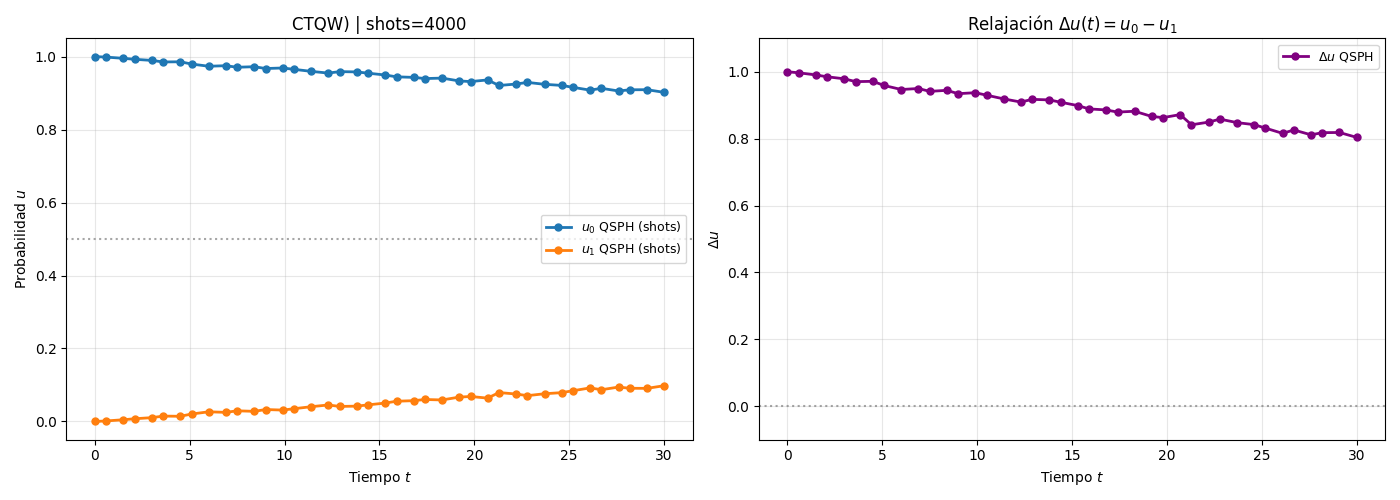
\includegraphics[width=0.95\textwidth]{chapters/cap5_circuito/img/sim_con_medida_inter.png}
    \caption{Evolución de las probabilidades del sistema tras introducir la interacción con el ancilla, la medición intermedia y el reinicio condicional. El patrón unitario se modifica, pero no aparece la relajación clásica.}
    \label{fig:sim-con-medida-inter}
\end{figure}

El circuito de un paso se muestra en la figura~\ref{fig:circ-medida-inter}, la cual consiste en el bloque de Matching Decomposition, $CX$ hacia el ancilla, medición intermedia y, si procede, $X$ de reinicio.

\begin{figure}[htbp]
    \centering
    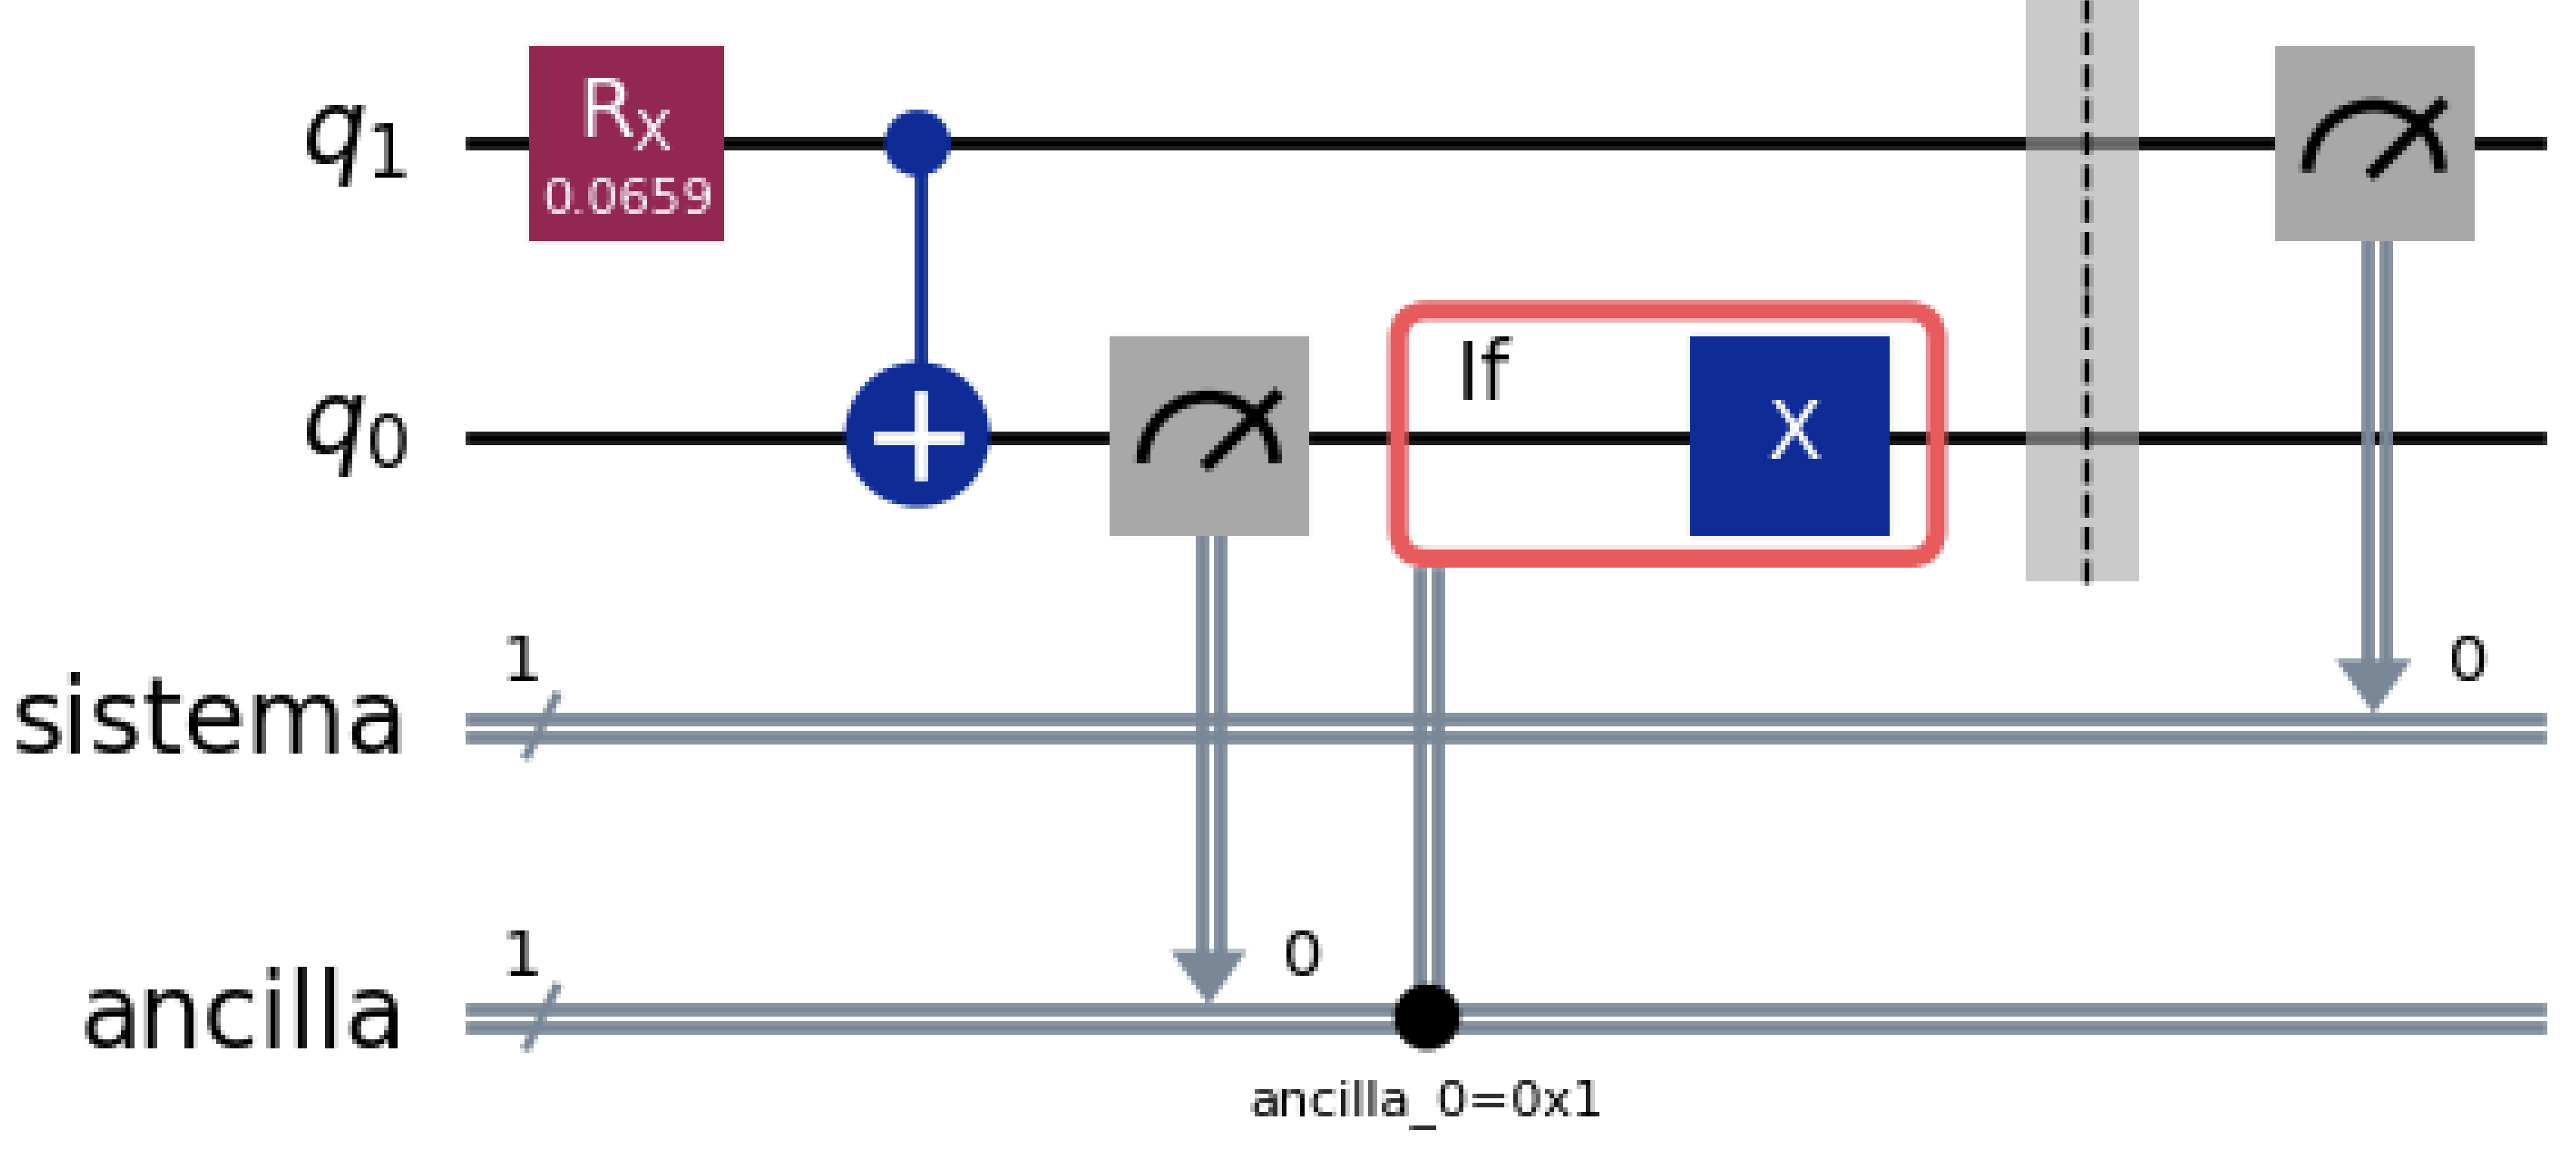
\includegraphics[width=\textwidth]{chapters/cap5_circuito/img/circ_medidainter.png}
    \caption{Circuito de un paso de Trotter con interacción sistema--ancilla, medición intermedia y reinicio condicional del ancilla.}
    \label{fig:circ-medida-inter}
\end{figure}

\section{Compensación del efecto Zeno}
\label{sec:compensacion-zeno}

La medición del ancilla en cada paso de Trotter no es neutra. Además de abrir el sistema, interrumpe la evolución coherente y puede reducir, o incluso congelar, la transferencia de amplitud entre partículas. Ese fenómeno es el efecto Zeno cuántico~\cite{nielsen2010,Kondo2016QZE}.

Para un sistema de dos niveles que parte de $\ket{0}$, un acoplamiento $J_{\mathrm{eff}}$ produce, en un intervalo $\Delta t$ y \emph{antes} de medir, la probabilidad de ocupación del segundo nodo~\cite{nielsen2010}
\begin{equation}
    P_{1}(\Delta t)
    =
    \sin^{2}\bigl(J_{\mathrm{eff}}\Delta t\bigr).
    \label{eq:probabilidad-transferencia-zeno}
\end{equation}
En el circuito cerrado esa expresión es la transferencia neta por paso. En el circuito abierto, la $CX$ y la medida del ancilla cortan esa evolución. Si $\Delta t$ es demasiado pequeño frente a $1/\Vert J\Vert$, el sistema apenas abandona $\ket{0}$ y la cantidad advectada queda prácticamente congelada~\cite{Kondo2016QZE}. Esa es la razón por la que la figura~\ref{fig:sim-con-medida-inter} no reproduce la relajación clásica de la figura~\ref{fig:cassical_sim}.

La compensación consiste en elegir $J_{\mathrm{eff}}$ de modo que la expresión \eqref{eq:probabilidad-transferencia-zeno} coincida con la probabilidad de transferencia del paso de Euler SPH. Si $J_{\mathrm{classic}}$ es el coeficiente de la matriz hermítica $J$, detallada en la sección \ref{sec:primera_implementacion}, se impone lo siguiente:

\begin{equation}
    \sin^{2}\bigl(J_{\mathrm{eff}}\Delta t\bigr)
    =
    J_{\mathrm{classic}}\Delta t,
    \label{eq:condicion-compensacion-zeno}
\end{equation}
de donde
\begin{equation}
    J_{\mathrm{eff}}
    =
    \frac{\arcsin\bigl(\sqrt{J_{\mathrm{classic}}\Delta t}\bigr)}{\Delta t},
    \qquad
    0\leq J_{\mathrm{classic}}\Delta t\leq 1.
    \label{eq:J-eff}
\end{equation}
La cota $J_{\mathrm{classic}}\Delta t\leq 1$ garantiza que el argumento de la raíz sea una probabilidad. Si se viola, hay que reducir $\Delta t$ aumentando el número de pasos de Trotter.

La expresión~\eqref{eq:J-eff} no aparece en la literatura de QSPH ni en los trabajos de Zeno citados, se trata de una calibración introducida en este trabajo. Lo que sí está en la literatura es el mecanismo que se corrige. La dependencia $\sin^{2}$ es la evolución unitaria de un sistema de dos niveles~\cite{nielsen2010}. La inhibición de esa evolución al medir con frecuencia es el efecto Zeno~\cite{Kondo2016QZE,Misra1977QZE}. La transformación $J\rightarrow J_{\mathrm{eff}}$ invierte localmente esa dependencia sinusoidal para que, una vez medida el ancilla, el salto por paso recupere la tasa clásica $J_{\mathrm{classic}}\Delta t$.

El hamiltoniano que entra en Matching Decomposition deja de ser la matriz $J$ de la ecuación~\eqref{mat: J} y pasa a ser
\begin{equation}
    J_{\mathrm{eff}}^{(\mathrm{mat})}
    =
    \begin{pmatrix}
        0 & J_{\mathrm{eff}}\\
        J_{\mathrm{eff}} & 0
    \end{pmatrix}.
    \label{eq:J-eff-matrix}
\end{equation}
La topología no cambia, sigue habiendo una única arista entre las dos partículas. Solo se reescala el acoplamiento.

Quedan, por tanto, dos piezas distintas. El ancilla, la $CX$, la medida y el reinicio abren el sistema~\cite{nielsen2010,Kondo2016QZE}. La sustitución~\eqref{eq:J-eff} no es una segunda fuente de disipación, es una corrección del acoplamiento para que el efecto Zeno no anule la tasa SPH. 

\section{Implementación final}

Con lo anterior se han definido todos los elementos necesarios para la implementación final, la evolución coherente mediante Matching Decomposition, la interacción sistema--ancilla mediante una puerta CNOT, la medición intermedia con reinicio condicional y la sustitución del acoplamiento original por el hamiltoniano efectivo $J_{\mathrm{eff}}$.

La última implementación combina estos componentes en cada paso de Trotter. Su objetivo es reproducir una transferencia compatible con la discretización clásica en el dímero $N=2$, sin mantener las oscilaciones indefinidas características del sistema cerrado. Los resultados numéricos, la comparación con la simulación clásica de la figura~\ref{fig:cassical_sim} y el análisis de la influencia de la frecuencia de medida se presentan en el capítulo~\ref{cap:resultados}.

